
%(BEGIN_QUESTION)
% Copyright 2007, Tony R. Kuphaldt, released under the Creative Commons Attribution License (v 1.0)
% This means you may do almost anything with this work of mine, so long as you give me proper credit

Determine how to adjust this bourdon-tube pressure gauge mechanism to correct for the calibration error exhibited in the ``As-Found'' calibration table.  

\vskip 10pt

\hbox{ % Encloses both image and table into a horizontal group

\includegraphics[width=15.5cm]{i03577x01.eps} \hskip 30pt

% No blank lines allowed between lines of an \halign structure!
% I use comments (%) instead, so that TeX doesn't choke.

%$$\vbox{\offinterlineskip
\vbox{\offinterlineskip
\halign{\strut
\vrule \quad\hfil # \ \hfil & 
\vrule \quad\hfil # \ \hfil \vrule \cr
\noalign{\hrule}
%
% First row
Applied pressure & Gauge indication \cr
%
(PSI) & (PSI) \cr
%
\noalign{\hrule}
%
% Another row
0 & 3 \cr
%
\noalign{\hrule}
%
% Another row
25 & 28 \cr
%
\noalign{\hrule}
%
% Another row
50 & 53 \cr
%
\noalign{\hrule}
%
% Another row
75 & 78 \cr
%
\noalign{\hrule}
%
% Another row
100 & 103 \cr
%
\noalign{\hrule}
} % End of \halign 
} % End of \vbox
%}$$ % End of \vbox

} % End of \hbox enclosing both image and table

\vskip 10pt

After inspecting the gauge, you see that you are able to adjust the following things:

\begin{itemize}
\item{} Lenghthen the ``link''
\item{} Shorten the ``link''
\item{} Move the pivot point between the ``link'' and the ``sector'' toward the pinion gear
\item{} Move the pivot point between the ``link'' and the ``sector'' away from the pinion gear
\item{} Shift the pointer clockwise on the ``pinion gear'' shaft
\item{} Shift the pointer counter-clockwise on the ``pinion gear'' shaft
\item{} Bend the bourdon tube upward (straighter)
\item{} Bend the bourdon tube downward (more bent)
\end{itemize}

\vskip 10pt

\noindent
Credit will be given for determining the following:

\begin{itemize}
\item{} Identify which piece of the mechanism to adjust to correct the gauge's calibration, and which way to adjust it (e.g. which direction to adjust the mechanism)
\vskip 5pt
\item{} Explain why this adjustment will work:
\end{itemize}

\underbar{file i03577}
%(END_QUESTION)





%(BEGIN_ANSWER)

\begin{itemize}
\item{} {\bf (5 points)} Identify which piece of the mechanism to adjust -- {\bf Either lengthen the link, or shift the pointer counter-clockwise on the ``pinion gear'' shaft.}
\vskip 5pt
\item{} {\bf (5 points)} Explain why this adjustment will work: {\bf Right now, we have a zero error, and it must be corrected by subtracting motion from the pointer.  The best fix for this is to remove and re-attach the pointer, but lenghtening the link will also work because it will offset the pointer's position.}
\end{itemize}

%(END_ANSWER)





%(BEGIN_NOTES)

{\bf This question is intended for exams only and not worksheets!}.

%(END_NOTES)


